\chapter{Vorbereitung}

\section{Theoretische Grundlagen zum AFM}
       
 \subsection{Aufbau des Rasterkraftmikroskops}
\begin{figure}[h!]
    \centering
    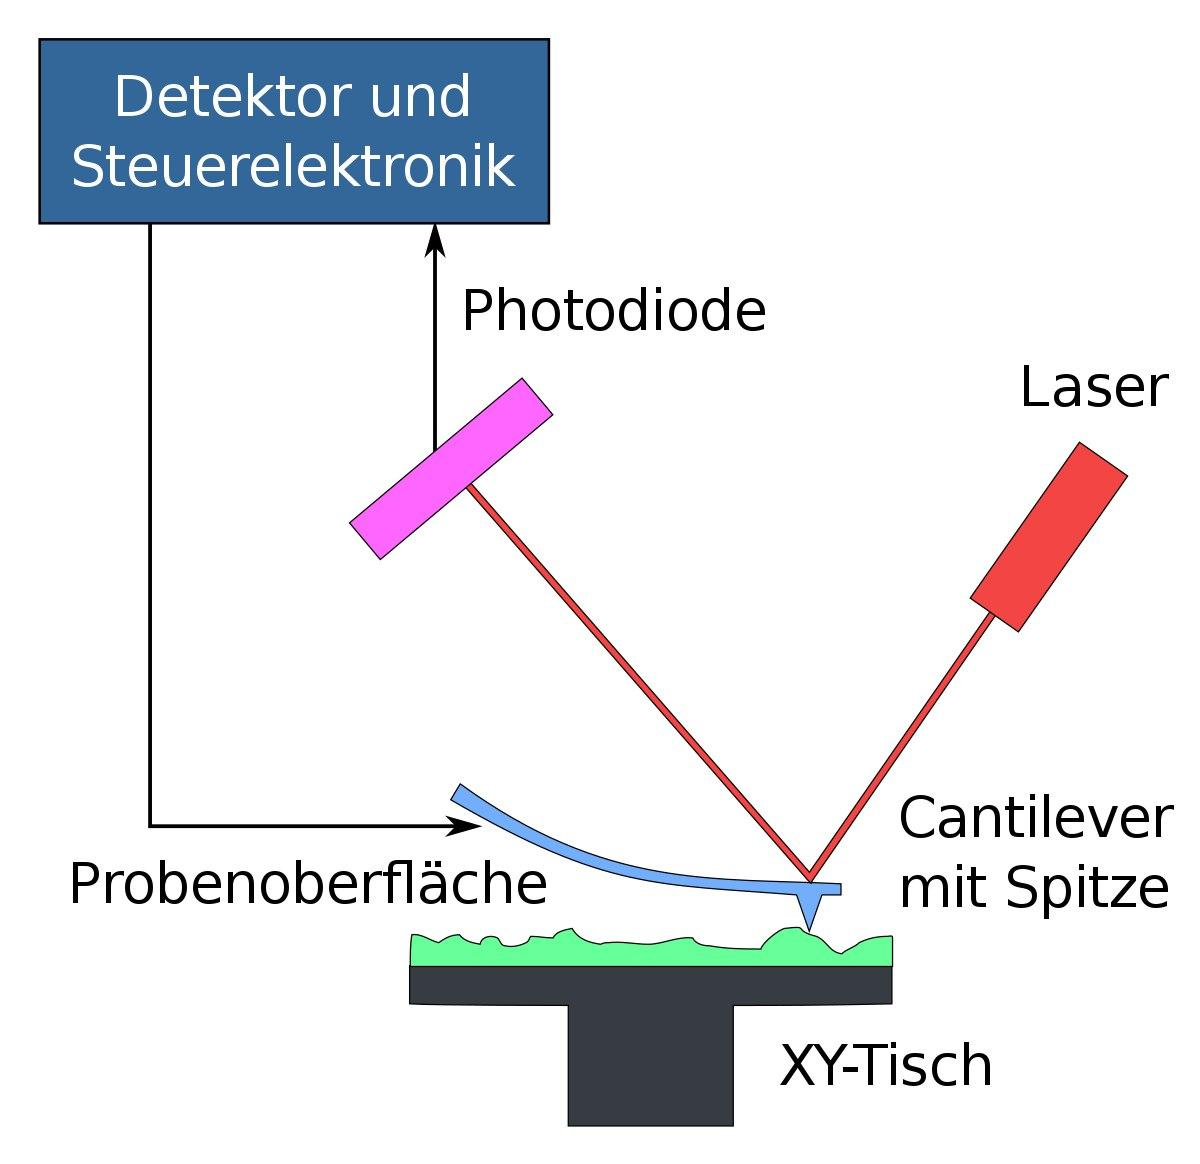
\includegraphics[width=0.6\textwidth]{Abb/afm.jpg}
    \caption{Aufbau eines AFM}
    \label{afm}
\end{figure}

Das Mikroskop besteht aus einem Cantilever mit Messspitze, einem Positioniersystem für die z-Richtung, einem Positioniersystem für x- bzw. y-Richtung und einer Detektionseinheit, welche die Amplitudenänderung des Cantilevers misst. 
Diese Bauteile sollen in den folgenden Kapiteln noch genauer beschrieben werden. 

 \subsection{Der Cantilever}
 
Der Cantilever ist ein schwingungsfähiger Balken, der eine pyramidale Spitze mit einer Dicke von nur wenigen Nanometern besitzt.
Er wird meist aus $Si_3N_4$ hergestellt und an dessen Ende wird, durch Ätzung, eine abstehende sehr sehr dünne Spitze geformt.
Seine Resonanzfrequenz befindet sich etwa im kHz bis MHz Bereich.
Damit lassen sich nun die Abstoßungs- bzw. Anziehungskräfte messen.
Man fährt den Cantilever mithilfe des Rastermechnismusses in nächster Nähe über die Probe.
Die Spitze wird mittels Schrittmotoren auf einen ungefähren Abstand von einem Mikrometer angenähert und anschließend über piezoelektrische Bauelemente weiter ausgerichtet, zu diesen später mehr.
Diese Vorrichtung führt letztendlich die Spitze über die Probe, in Entfernungen von 10 - 100 Mikrometern in x- und y-Richtung und einer Höhe von unter 10 Mikrometern.
Gleichzeitig versetzt man den Cantilever in seine Resonanzfrequenz und beobachtet über die Detektionseinheit, wie stark diese Schwingung durch den Abstand zur Probe eingeschränkt wird.

 \subsection{Detektionseinheit}
 
 Das in diesem Versuch verwendete EasyScan DFM Rasterkraftmiskroskop nutzt zur Auslesung der Amplitudenänderung ein optisches Verfahren. 
 Man verwendet einen Laser, der auf die Rückseite des Cantilevers ausgerichtet ist, wo sich eine polierte Stelle befindet, welche das Licht des Lasers spiegelt.
 Bei der Deformation des Cantilevers ändert sich somit die Position des gespiegelten Lichtbündels.
 Mithilfe einer Photodiode lassen sich diese minimalen Änderungen sehr gut messen und in Größenordnungen von einzelnen Angstrøm umrechnen.
 Diese Methode eignet sich hervorragend, denn das Laserlicht wird lediglich durch Erschütterungen gestört.
 Deshalb baut man diesen Versuch auf einem massiven Steintisch auf und versucht Erschütterungen bei der Messung zu vermeiden.

\subsection{Rastermechanismus}

Nun muss noch beschrieben werden, wie es sich mit der Rastereinheit verhält.
Am Anfang fährt man die Probe mittels eines Schrittmotors mechanisch bis auf wenige Mikrometer auf die Probe in z-Richtung heran.
Anschließend nutzt man den piezoelektrischen Effekt um eine feinere Ansteuerungen zu ermöglichen.
Zumeist verwendet man piezoelektrische Röhrchen aus Blei-Zirkonat-Titanat, denn dieses Material kann sich mithilfe einer angelegten Spannung stark dehnen und zusammenziehen. 
Typische Rasterbereiche sind $10-\SI{100}{\mu m}$ in x- und y-Richtung und $2-\SI{5}{\mu m}$ in z-Richtung.
Das hier verwendete Mikroskop basiert auf diesem elektromechanischem Prinzip, also der Deformierung der piezoelektrischen Materialien zur feineren Bewegung des Cantilevers.
Alternativ lässt sich auch die Probe bewegen.

\subsection{Betriebsmodi}

Es gibt zwei Methoden zur Messung, den statischen Modus und den dynamischen Modus. Beim statischen Modus wird der Cantilever nicht in Schwingung versetzt, beim dynamischen hingegend schon. Der statische Modus ist nur von historischer Bedeutung.

\paragraph{Statischer Modus:}

Hierbei bringt man die Probe mit dem Cantilever in Kontakt und misst die direkte Kraft, die der Cantilever beim abrastern der Probenoberfläche erfährt. 
Die Kräfte die zwischen dem Cantilever und der Probe auftreten, sollen später noch genauer betrachtet werden.
Die Rastereinheit regelt die z-Position gerade so, dass sich Probe und Cantilver ständig berühren.
Da sich hierbei aber die Probe und der Cantilever schnell abnutzen, wurde der 
dynamische Modus als Alternative eingeführt.

\paragraph{Dynamischer Modus:}

Dazu versetzt man den Cantilever, nach dem Prinzip der harmonischen Schwingung, in seine Eigenresonanz.
Die im nächsten Kapitel besprochenen Kräfte ändern nun die Schwingungsfrequenz und Schwinungsamplitude.
Um einfache Ergebnisse erzielen zu können, kann man einerseits den Cantilever ständig in seine Resonanzfrequenz versetzen und die Änderung der Schwingungsamplitude messen, oder eine Phasenverschiebung der Anregungsfrequenz mit der Antwort des Cantilevers abgleichen.
Mit diesem eindeutigen Ergebnis lässt sich anschließend die Topologie der Probe rekonstruieren ohne dabei die Probe zu zerstören.
\vspace{6pt}\\
In unserem Versuch wird die Methode der Amplitudenänderung verwendet. 
Die anziehenden und abstoßenden Kräfte deformieren den Cantilever so stark, dass der Weg des Lasers im Angström Bereich umgelenkt wird. 
Eine Amplitudenänderungen von 70\%, zur Resonanzamplitude, ist maximal. 


    \section{Kräfte zwischen Atomen}
        \subsection{Van-der-Waals Kräfte}

Die Ladungsverteilung in Atomen ist nicht konstant, sondern unterliegt ständiger 
Fluktuation. Der Schwerpunkt der negativen Ladungen kann hierbei vom dem der
positiven Ladungen abweichen. Ist dies der Fall, so entsteht ein Dipol. 
Befindet sich nun ein zweites Teilchen in der Nähe dieses Atoms, so wird auch
in diesem ein Dipol induziert. Zeigt die positive Seite des ersten Atoms zu Atom 2,
so werden die Elektronen des zweiten Atoms angezogen. Ist es die negative Seite, so
werden die Elektronen abgestoßen. 
\vspace{3pt}\\
Als Folge dessen synchronisieren sich die Ladungsänderungen der beiden Atome. Eine
schwache positive Anziehung ist die Folge. Diese ist proportional zu $\displaystyle
\frac{-1}{r^6}$.

        \subsection{Pauli-Abstoßung}

Nähern sich die Atome weiter an, so kommt es zu einem Überlappen der 
Elektronenorbitale. Das Pauli-Verbot verhindert hierbei, dass zwei Elektronen den
gleichen Zustand besetzen. Einige Elektronen werden folglich in einen energetisch
höheren Zustand gezwungen. \\
So führt eine Orbitalüberlagerung zu einer repulsiven Wechselwirkung. Die Kraft
ist proportional zu $\displaystyle \frac{1}{r^{12}}$.

        \subsection{Lennard-Jones Potential}

Bei sehr kleinen Abständen dominiert die Pauli-Abstoßung, bei größeren die 
van-der-Waals Kräfte. Die Summe aus beiden Potentialen wird Lennard-Jones 
Potential gennant. 
\[
   \phi (r) \propto \frac{A}{r^6} - \frac{B}{r^{12}}    
\]

Dabei bezeichnet $\phi$ das Potential und somit die Bindungsenergie, r den Abstand.
A, B sind Konstanten die stoffspezifisch sind.

\begin{figure}[h!]
    \centering
    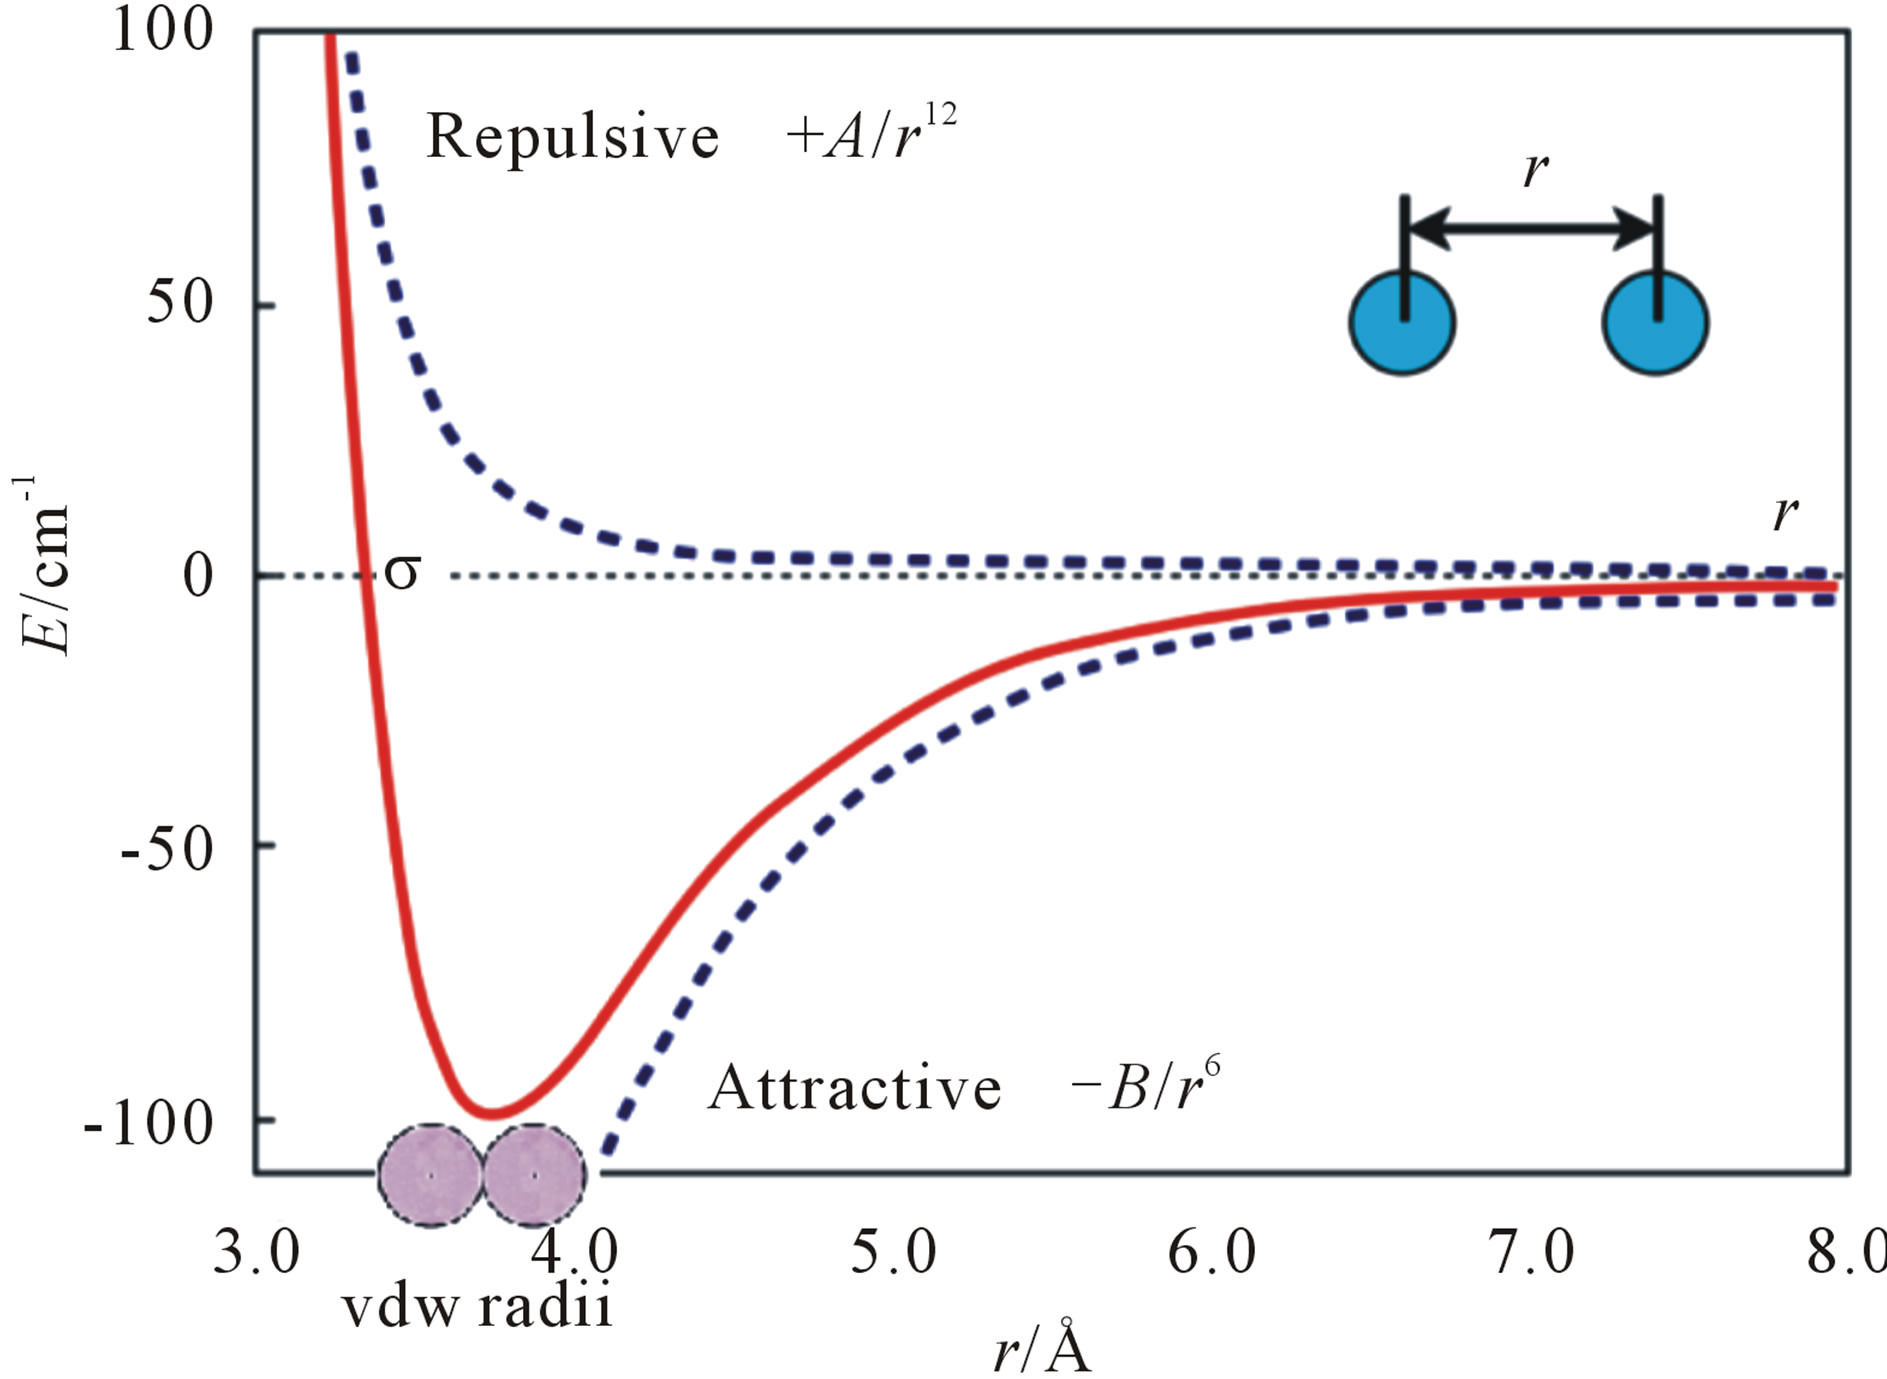
\includegraphics[width=0.6\textwidth]{Abb/ljp.jpg}
    \caption{Das Lennard-Jones Potential als Summe der vdW-Wechselwirkung und
             der Pauli-Abstoßung}
    \label{ljp}
\end{figure}

Neben diesen Kräften können im Allgemeinen auch noch chemische Bindungskräfte, Kontaktkräfte, magnetische und elektrische Wechselwirkungen eine Rolle besitzen.
Bei unserem Aufbau haben sie jedoch nur geringe Bedeutung.

 
\section{Berechnung der Amplitude}
\label{herleitung}
 
Die periodische Bewegung des Cantilevers lässt sich in sehr guter Näherung durch einen getriebenen, gedämpften harmonischen Oszillator beschreiben. Die Formel dazu sieht folgendermaßen aus:
\[
    m \ddot{x} + \frac{m \omega_0}{Q} \dot{x} + kx = F_0 \cos(\omega t)
\]
Wir verwenden hier m als die punktförmig genäherte Masse des Cantilevers, $\omega_0$ ist dessen Eigenfrequenz mit seiner Güte $Q$ und $k$ beschreibt eine Federkonstante die für die rücktreibende Kraft, also die Oszillation, verantwortlich ist.
Auf der rechten Seite der Gleichung beschreibt $F_0$ die treibende Kraft, die die Probe und die Vorrichtung auf den Cantilever wirken.
Wir benutzen den Ansatz:
\[
    x(t)=A \cdot e^{iwt}
\]
und bekommen schließlich durch Einsetzen folgende Gleichung.
\[
   \left(-\omega^2+\omega_0^2-i\frac{\omega_0}{Q} \cdot \omega \right) \cdot A 
   = \frac{F_0}{m}
\]
Löst man diese Gleichung anschließend nach der Amplitude A auf, erhält man 
folgendes Ergebnis:
\[
    A = \frac{F_0}{m \sqrt{ ( \omega_0^2 - \omega^2 )^2 + \left( \frac{\omega 
        \omega_0}{Q} \right)^2}}
\]
Diese Formel ist später für unseren Versuch noch von Bedeutung.
